\documentclass[12pt]{kiarticle}
\DeclareGraphicsExtensions{.pdf,.png,.jpg,.eps}
%%%
\pagestyle{fancy}
\fancyhf{}
%\renewcommand{\headrulewidth}{ 0.1mm }
\renewcommand{\footrulewidth}{ .0em }
\fancyfoot[C]{\texttt{\textemdash~\thepage~\textemdash}}
\fancyhead[L]{Лабораторная работа № 4.7.2 \hfil}
\fancyhead[R]{\hfil Иванов Кирилл, 625 группа }
\usepackage{multirow} % Слияние строк в таблице
\newcommand
{\un}[1]
{\ensuremath{\text{#1}}}
\newcommand{\eds}{\ensuremath{ \mathscr{E}}}
\usepackage{tikz}
%%% Работа с таблицами
\usepackage{array,tabularx,tabulary,booktabs} % Дополнительная работа с таблицами
\usepackage{longtable}  % Длинные таблицы
\usepackage{multirow} % Слияние строк в таблице
\usepackage{pgfplotstable}
\usepackage{longtable}
%\usetikzlibrary{shapes.multipart}
% Листинги
\usepackage{moreverb}
\usepackage{listings}
\lstset{
	frame=single,
	showspaces=false,
	showstringspaces=false,
	numbers=left,
}

% Среднее значение
\newcommand{\aver}[1]{\langle #1 \rangle}

% Таблицы
\usepackage{multirow}
\usepackage{hhline}
\usepackage{makecell}
\title{Лабораторная работа 4.7.2 \\ Эффект Поккельса}

\newcommand{\specialcell}[2][c]{%
	\begin{tabular}[#1]{@{}c@{}}#2\end{tabular}}

\renewcommand{\thesubsection}{\arabic{subsection}}

\begin{document}
	
		\begin{titlepage}
		\begin{center}
			\large 	Московский физико-технический институт \\
			(государственный университет) \\
			Факультет общей и прикладной физики \\
			\vspace{0.2cm}
			
			\vspace{4.5cm}
			Лабораторная работа № 4.7.2 \\ \vspace{0.2cm}
			\large (Общая физика: оптика) \\ \vspace{0.2cm}
			\LARGE \textbf{Эффект Поккельса}
		\end{center}
		\vspace{2.3cm} \large
		
		\begin{center}
			Работу выполнил: \\
			Иванов Кирилл,
			625 группа
			\vspace{10mm}		
			
		\end{center}
		
		\begin{center} \vspace{60mm}
			г. Долгопрудный \\
			2018 год
		\end{center}
	\end{titlepage}
	
	
		\paragraph*{Цель работы}: исследовать интерференцию рассеянного света, прошедшего кристалл; наблюдать изменение характера поляризации света при наложении на кристалл электрического поля.
	
		\paragraph*{Оборудование:} гелий-неоновый лазер, поляризатор, кристалл ниобата лития LiNbO$_3$, матовая пластинка, экран, источник высоковольтного переменного и постоянного напряжения, фотодиод, осциллограф, линейка.
	
	Рассмотрим кристалл ниобата лития: его оптические свойства обладают симметрией вращения относительно выделенного направления - оптической оси $Z$. Для волны, распространяющейся вдоль $Z$, показатель преломления равен $n_e$, а для волны, перпендикулярной оптической оси, - $n_o$, причем $n_o > n_e$. Волну длины $\lambda = 2\pi/k$, проходящую под углом $\theta$ к оси $Z$ в кристалле, принято раскладывать на обыкновенную и необыкновенную. Для вектора напряженности обыкновенной волны верно: $\overrightarrow{E_o} \perp (\overrightarrow{k}, \overrightarrow{Z})$, - и показатель преломления равен $n_0$. Для вектора напряженности необыкновенной: $\overrightarrow{E_e} \in (\overrightarrow{k}, \overrightarrow{Z})$, - и показатель преломления $n_2$ зависит от $\theta$ по закону:
	
	\[ \frac{1}{n_2^2} = \frac{\cos^2\theta}{n_o^2} + \frac{\sin^2\theta}{n_e^2} \]
	
	Разность хода обыкновенной и необыкновенной волн при прохождении кристалла длиной $l$ составляет: 
	
	\[ \Delta = kl(n_0 - n_2) = \frac{2\pi}{\lambda} \cdot l (n_0 - n_2) \]
	
	С учетом зависимости $n_2(\theta)$ для малых углов $\theta$ в приближении $n_o \approx n_e$: 
	
	\begin{equation}
		\Delta = \frac{2\pi}{\lambda}\cdot l (n_o - n_e)\theta^2 
	\end{equation}
	
	\begin{wrapfigure}{r}{0.4\linewidth} 
		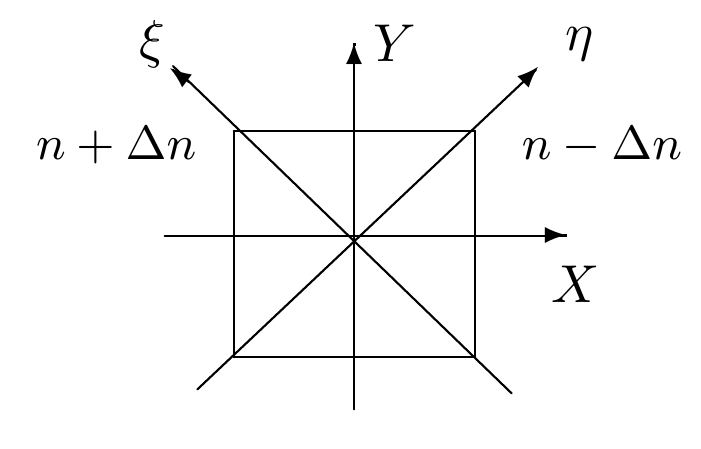
\includegraphics[width=\linewidth]{maindir}
		\caption{Эффект Поккельса: главные направления при наложении электрического поля}
		\label{dir}
	\end{wrapfigure}
	
	Направления постоянной разности фаз задают косинусы $\cos\theta$, следовательно, интерференционная картина являет концентрические окружности. 
	
	Поместим кристалл ниобата лития в постоянное электрическое поле $E_{el}$, направленное по оси $X$, перпендикулярной оптической оси $Z$. В плоскости $(\overrightarrow{X}, \overrightarrow{Y})$ возникают быстрая и медленная оси под углами $45^\circ$ к $X$, $Y$, соответствующие показателям преломления $(n_o - \Delta n)$ и $(n_o + \Delta n)$, здесь $\Delta n = A\cdot E_{el}$, $A$ - константа, зависящая от свойств материала. В этом и заключается \textbf{эффект Поккельса}. 
	
	Появление главных направлений $\xi$ и $\eta$ иллюстрирует рисунок \ref{dir}. 
	
	\subsection{Исследование интерференции рассеянного света}
	
	Схема наблюдения интерференционной картины приведена на рисунке \ref{shema}. Свет лазера, поляризованный в вертикальной плоскости, рассеивается на матовой пластинке и проходит через двоякопреломляющий кристалл. На выходе из кристалла стоит поляроид. Параметры установки: размеры кристалла $3 \times 3 \times 26$ мм, длина волны гелий-неонового лазера $\lambda = 0,63$ мкм, показатель преломления $n_o = 2,29$, расстояние до экрана от центра кристалла $L = (76 \pm 1)$ см. 
	
	\begin{figure}[h]
		\centering	
		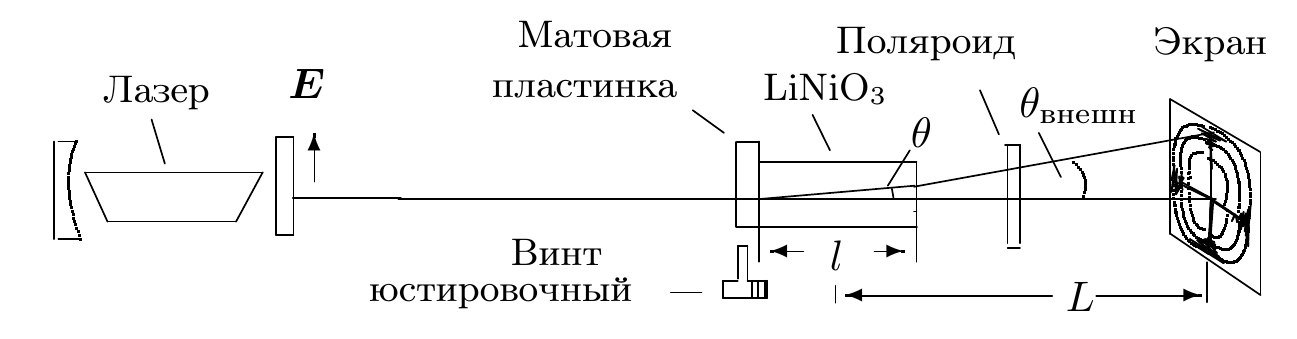
\includegraphics[width=0.6\textwidth]{shema.png}
		\caption{Схема наблюдения интерференционной картины}
		\label{shema}
	\end{figure}
	
	Интерференционная картина, создаваемая обыкновенной и необыкновенной волнами, наблюдается в скрещенной поляризации. Для луча, идущего вдоль оптической оси $Z$, верно: $n_o = n_e$; его поляризация не изменяется в кристалле, луч не проходит через анализатор, и в центре интерференционной картины находится темное пятно. Следующий минимум интенсивности соответствует сдвигу фаз между волнами на $2\pi$, поэтому условие на $m$-ое темное кольцо запишется с использованием формулы (1) в виде:
	
	\[ \Delta = 2\pi m \leftrightarrow \frac{2\pi}{\lambda}\cdot l (n_o - n_e)\theta_m^2 = 2\pi m \leftrightarrow \theta_m^2 = \frac{m\lambda}{l(n_o - n_e)} \] 
	
	Здесь $l = 26$ мм - длина кристалла вдоль оптической оси.
	
	По закону Снеллиуса, угол преломления на внешней границе кристалла: $\theta_{ex} = n_o\theta$. Тогда для радиуса $m$-ого темного кольца $r_m$ верно: 

	\begin{equation}	
		r_m^2 = \frac{\lambda}{l} \frac{(n_oL)^2}{(n_o - n_e)} \cdot m
	\end{equation}
	
	Соберем установку по схеме на рисунке \ref{shema}, предварительно убедившись в вертикальной поляризации лазера. Лазер установим так, чтобы в отсутствии кристалла излучение через него не проходило. Оптимальное расстояние $L$ от экрана до центра кристалла определим экспериментально, центр интерференционной картины совместим с изображением луча в отсутствие матовой пластинки. При повороте анализатора на $90^\circ$ градусов от исходного положения картинка на экране меняется на негативную, что соответствует смене разрешенной выходной поляризации и, следовательно, условиям на темные кольца. 
	
	Снимем зависимость радиусов темных концентрических колец от номера максимума $r_m(m)$. Для большей точности измерений отметим положения колец на экране вдоль прямой карандашом. Погрешность величины $r_m$ примем равной $0,2$ см из-за расплывчатости картинки. Результаты измерений занесены в таблицу \ref{circles}. 
	
	\begin{table}[h]
		\centering
		\begin{tabular}{|c|c|c|c|c|c|c|c|c|c|}
\hline
$m$&1&2&3&4&5&6&7\\
\hline
$r_m$, см&2,7&3,7&4,9&5,6&6,3&7,1&7,5\\
\hline
$r_m^2$, $\text{см}^2$&7,3&13,7&24,0&31,4&39,7&50&56\\
\hline
$\Delta r_m^2$, $\text{см}^2$&0,8&1,0&1,4&1,6&1,8&2&2\\
\hline
\end{tabular}
		\caption{Измерение квадратичной зависимости радиуса темного кольца интерференционной картины от номера минимума}
		\label{circles}
	\end{table}	
	
	На основе таблицы \ref{circles} построен график зависимости квадрата радиуса кольца от номера соответствующего минимума $r_m^2(m)$, изображенный на рисунке \ref{r(m)}. Погрешность $r_m^2$ рассчитана по формуле произведения погрешностей. 
	
	\begin{figure}[h]
		\centering
		
		\pgfplotstableread {
			x			y			xerr		yerr
			1			7.3			0			0.8
			2			13.7		0			1.0
			3			24.0		0			1.4
			4			31.4		0			1.6
			5			39.7		0			1.8
			6			50			0			2
			7			56			0			2
		}\datatable
		\pgfplotstablecreatecol[linear regression={y=y}]{regression}{\datatable}
		\xdef\coefA{\pgfplotstableregressiona} % save the slope parameter
		\xdef\coefB{\pgfplotstableregressionb} % save the intercept parameter
		
		\begin{tikzpicture}
		
		\begin{axis}[width = 0.6\textwidth, 
		%axis lines = middle,
		%axis line style = thick,
		xlabel = {$m$},
		ylabel = {$r_m^2$, $\text{см}^2$},
		legend pos=outer north east,
		%every axis x label/.style={at={(current axis.right of origin)},anchor=north west},
		%every axis y label/.style={at={(current axis.above origin)},anchor=north east},	
		]
		
		\addplot[only marks,
		mark size=1,
		black,
		error bars/.cd,
		x dir = both, x explicit,
		y dir = both, y explicit,
		] table
		[x=x, y=y, x error = xerr, y error = yerr ]
		{	
			x			y			xerr		yerr
			1			7.3			0			0.8
			2			13.7		0			1.0
			3			24.0		0			1.4
			4			31.4		0			1.6
			5			39.7		0			1.8
			6			50			0			2
			7			56			0			2
		};
		
		\addplot [thick, no markers, domain=0:8] {\coefA*x + \coefB};
		
		\node at (500, 30) {\begin{tabular}{c} $r_m^2 = bm + a$ \\ $b = (8,43 \pm 0,19) \text{ см}^2$ \end{tabular}};

		\end{axis}
		\end{tikzpicture}
		\caption{График зависимости квадрата радиуса темного кольца интерференционной картины от номера минимума $r_m^2(m)$}
		\label{r(m)}
	\end{figure}
	
	Экспериментальные точки хорошо на прямую $r_m^2 = bm + a$, что соответствует теоретической зависимости (2). Проведем ее методом наименьших квадратов, воспользовавшись привычными формулами для коэффициентов прямой и их погрешностей.
	
	Для коэффициента наклона имеем: 
	
	\[ b = \frac{\lambda}{l} \frac{(n_oL)^2}{(n_o - n_e)} = (8,43 \pm 0,19) \text{ см}^2 \] 
	
	Выразим двулучепреломление ниобата лития $n_o - n_e$:
	
	\[ n_o - n_e = \frac{\lambda}{l}\frac{(n_oL)^2}{b} = (87 \pm 3) \cdot 10^{-3} \]
	
	Для вычисления использовались параметры установки, описанные в начале раздела. Считаем, что вклад в погрешность дают непосредственно измеренные величины: длина от центра кристалла до экрана $L$ и коэффициент $b$.
	
	\subsection{Изменение характера поляризации света \\ при наличии внешнего поля}
	
	При наложении электрического поля в кристалле возникают быстрая ось $\xi$ и медленная ось $\eta$, изображенные на рисунке \ref{dir}; разложим вектор напряженности волны по ним. После прохождения кристалла разность фаз между $E_\eta$ и $E_\xi$ составит $\Delta = \frac{2\pi}{\lambda} \cdot2l\Delta n = \frac{4\pi}{\lambda} \frac{l}{d} AU$, где $U = E_{el}d$ - напряжение на кристалле, $d = 3$ мм - его поперечный размер, $l = 26$ мм - длина пути луча. Поляроид пропускает горизонтальную составляющую волны. Значит, выходная напряженность складывается из проекций $E_\eta$ и $E_\xi$ на ось $X$:
	
	\[ E = \frac{E_0}{2} \cdot e^{i(\omega t - kl)} (e^{i\Delta/2} - e^{i\Delta/2}) = \frac{E_0}{2} \cdot  e^{i(\omega t - kl + \pi/2)} \sin\frac{\Delta}{2} \]
	
	Здесь $E_0$ - амплитуда входной волны.
	
	Отсюда интенсивность выходной волны: 
	
	\begin{equation}
		I = I_0 \sin^2\frac{\Delta}{2} = I_0\sin^2 \left(\frac{\pi}{2}\frac{U}{U_{\lambda/2}}\right) 
	\end{equation}
	
	Здесь введено \textbf{полуволновое напряжение} $U_{\lambda/2} = \frac{\lambda}{4A}\frac{d}{l}$, соответствующее максимальной интенсивности на выходе.
	
	При параллельных поляризациях лазера и анализатора получаем следующую зависимость $I(U)$:
	
	\begin{equation}
		I = I_0 \cos^2\left(\frac{\pi}{2}\frac{U}{U_{\lambda/2}}\right)
	\end{equation} 
	
	Полная схема установки, включающая блок питания, фотодиод и осциллограф, используемые в этой части работы, показана на рисунке \ref{full}. 
	
	\begin{figure}[h]
		\centering	
		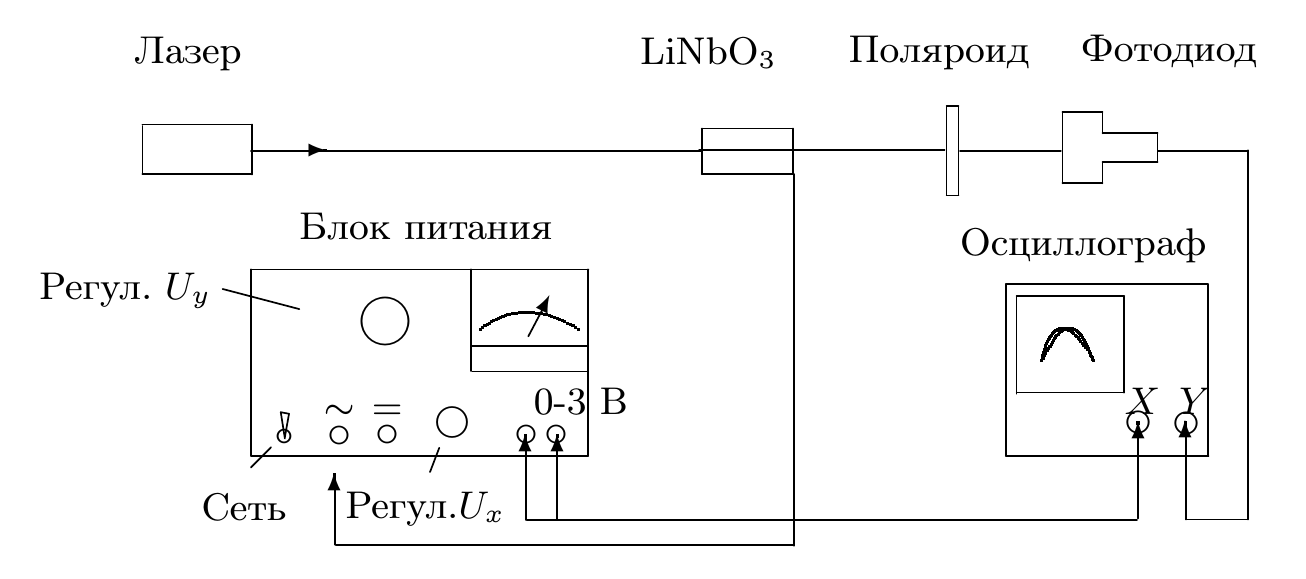
\includegraphics[width=0.6\textwidth]{fullpic.png}
		\caption{Схема установки для изучения двулучепреломления в электрическом виде}
		\label{full}
	\end{figure}
	
	Соберем схему как на рисунке \ref{full} и подключим разъем блока питания на постоянное напряжение. Увеличивая напряжение с нулевого значения, проследим за изменением яркости пятна на экране. 
	
	Для скрещенных поляризаций при напряжениях $U = (2k - 1)U_{\lambda/2}$ наблюдается максимум интенсивности, при $U = 2kU_{\lambda/2}$ - минимум, здесь $k$ - натуральное число. Для параллельных поляризаций ситуация противоположная. 
	
	Напряжения, соответствующие последовательным экстремумам интенсивности для разных поляризаций, содержатся в таблице \ref{vol}.	В 100 делениях шкалы блока питания 1,5 кВ. Погрешность измерения напряжения примем равной 1 делению, или 15 В. 
	
	\begin{table}[h]
		\centering
		\begin{tabular}{|c|c|c|}
\hline
&Скрещенные поляризации&Параллельные поляризации\\
\hline
$U_{\lambda/2}$, дел&30&28\\
\hline
$U_{\lambda/2}$, В&450&420\\
\hline
\hline
$2U_{\lambda/2} = U_\lambda$, дел&60&60\\
\hline
$2U_{\lambda/2} = U_\lambda$, В&900&900\\
\hline
\hline
$3U_{\lambda/2} = U_{3\lambda/2}$, дел&92&92\\
\hline
$3U_{\lambda/2} = U_{3\lambda/2}$, В&1380&1380\\
\hline
\end{tabular}
		\caption{Измерение последовательных напряжений, соответствующих минимумам/максимумам интенсивности для скрещенных и параллельных поляризаций}
		\label{vol}
	\end{table}	
	
	По таблице \ref{vol} найдем среднее значение полуволнового напряжения; погрешность его определения складывается из приборной погрешности и случайной, сопоставимых по величине, поэтому оценим ее как $2\cdot 10$ В. 
	
	\[ U_{\lambda/2} = (46 \pm 2) \cdot 10 \text{ В} \] 
	
	При напряжении $U_{\lambda/4}$ интенсивности при скрещенной и параллельной поляризациях совпадают. Выставим экспериментальное значение напряжения $U_{\lambda/4} = U_{\lambda/2}/2 \approx 230$ В. При вращении анализатора интенсивность наблюдаемого пятна практически не меняется, что свидетельствует о круговой поляризации и подтверждает правильность расчетов.  
	
	Заменим в схеме, изображенной на рисунке \ref{full}, экран фотодиодом, подключим его к $Y$-входу осциллографа. На $X$-вход подадим переменное напряжение с блока питания. В режиме DUAL на экране осциллографа получаются фигуры Лиссажу, отвечающие зависимости $I(U)$. Она задается формулой (3) для скрещенных поляризаций и имеет вид синусоиды, взятой на симметричном отрезке, или формулой (4) для параллельных поляризаций и представляет собой косинусоиду. Таким образом, фигуры Лиссажу для разных поляризаций при одинаковом значении амплитуды напряжения $U$ отличаются по фазе на $\pi/2$.
	
	Определим полуволновое напряжение, измерив разность показаний между последовательными фигурами Лиссажу на экране, соответствующие экстремумам сигнала: 
	
	\[ U_{\lambda/2} \approx 30 \text{ дел} = 450 \text{ В} \]
	
	Фотографии наблюдаемых фигур Лиссажу для напряжений, кратным полуволновому, при параллельных поляризациях представлены на рисунке \ref{lis}.
	
	\textbf{Вывод:} 1) в работе изучена интерференция рассеянного света, прошедшего кристалл ниобата лития: получена зависимость квадрата радиуса темного кольца интерференционной картины от номера минимума $r_m^2(m)$, с хорошей точностью являющаяся линейной (ошибка углового коэффициента 2\%), что согласуется с теорией при малых углах отклонения луча от оптической оси кристалла и близких значениях показателей преломления для обыкновенной и необыкновенной волн. Действительно, двулучепреломление кристалла $n_o - n_e$ составляет $(87 \pm 3)\cdot10^{-3}$, это значение соответствует литиевым кристаллам. 2) Рассмотрен эффект Поккельса: несколькими способами определено полуволновое напряжение, оно совпадает в пределах погрешности и равно $U_{\lambda/2} \approx 460$ В. Получены фигуры Лиссажу, отражающие зависимость интенсивности выходного сигнала от подаваемой амплитуды напряжения $I(U)$ при скрещенных и параллельных поляризациях. Картинки для поляризаций отличаются по фазе на $\pi/2$.
	
	\begin{figure}[h]
		\begin{minipage}[h]{0.3\linewidth}
			\center{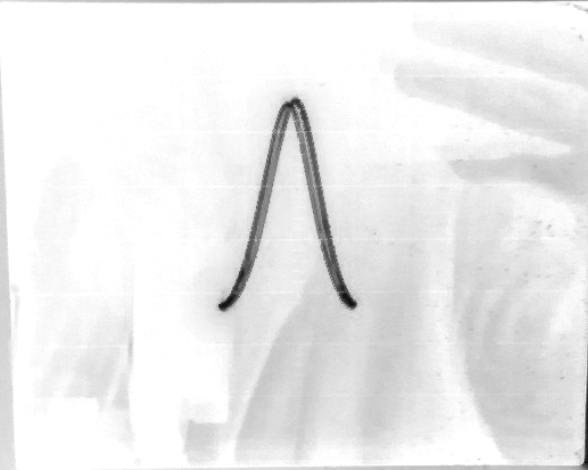
\includegraphics[width=0.9\linewidth]{photo1.png} \\ a)}
		\end{minipage}
		\hfill
		\begin{minipage}[h]{0.3\linewidth}
			\center{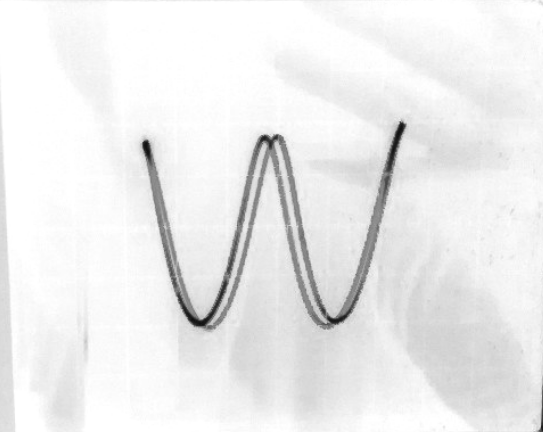
\includegraphics[width=0.9\linewidth]{photo2.png} \\ b)}
		\end{minipage}
		\hfill
		\begin{minipage}[h]{0.3\linewidth}
			\center{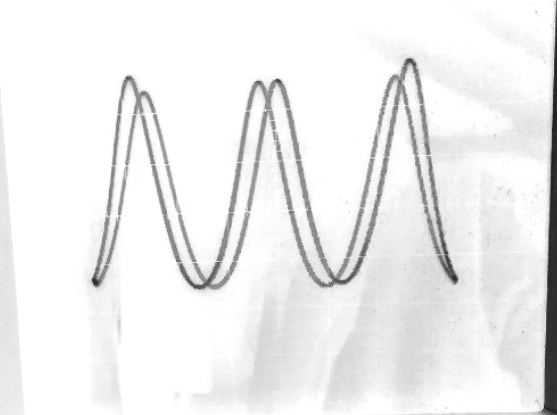
\includegraphics[width=0.9\linewidth]{photo3.png} \\ c)}
		\end{minipage}
		\caption{Фигуры Лиссажу для параллельных поляризаций при различных амплитудах напряжения $U$: (a) $U = U_{\lambda/2}$, (b) $U = U_{\lambda}$, (c) $U = U_{3\lambda/2}$ }
		\label{lis}
	\end{figure}
	
\end{document}